% =========================================================================================
% Title -------------+ Shakudo-Crucible Architecture
% Course ------------+ CS 4792 - Senior Design II
% Semester ----------+ Fall 2026
% Description -------+ This document is used as a visualization of the software system
%                      architecture. 
% AI Disclosure -----+ This document was planned out manually with preliminary LaTeX 
%                      code / diagrams made by hand. Generative AI was used to improve
%                      visuals and offer suggestions for wording.        
% Notes -------------+ This document (as of 10/21/2026) assumes a single merged
%                      aSketch-API.jar. AlloyIntegration.ts and
%                      blockly_alloy_integration.jar no longer exist.
%
% =================================== - VERSIONS - ========================================
%   v1.0            >> DATE: 10/17/2026  -  AUTHOR: Caden Rose
%                      --------------------------------------------------------------------
%                   >> Document creation for two JAR file architecture.
% =========================================================================================
%   v1.1            >> DATE: 10/21/2026  -  AUTHOR: Caden Rose
%                      --------------------------------------------------------------------
%                   >> Merged blockly-alloy-integration into aSketch-API and removed
%                      AlloyIntegration.ts. Run now goes main.ts -> crucibleApi.ts ->
%                      POST /shakudo.
% =========================================================================================
%   v1.2            >> DATE: 10/26/2026  -  AUTHOR: Kyler Hillstrom
%                      --------------------------------------------------------------------
%                   >> Added project IPC (crucible:list-projects, create-project,
%                      open-project, delete-project, select-alloy-file) and the
%                      projects-changed push. File > Open and crucible:open-project both
%                      go through openProject() in main.ts.
% =========================================================================================
\documentclass{article}

\usepackage[landscape,margin=0.6in]{geometry}
\usepackage{tikz}
\usetikzlibrary{arrows.meta,positioning,fit,backgrounds,calc}

\begin{document}
\thispagestyle{empty}

\begin{center}
\textbf{Shakudo--Crucible Architecture} \\
CS 4792 -- Senior Design II \\
Fall 2026
\end{center}

\begin{center}
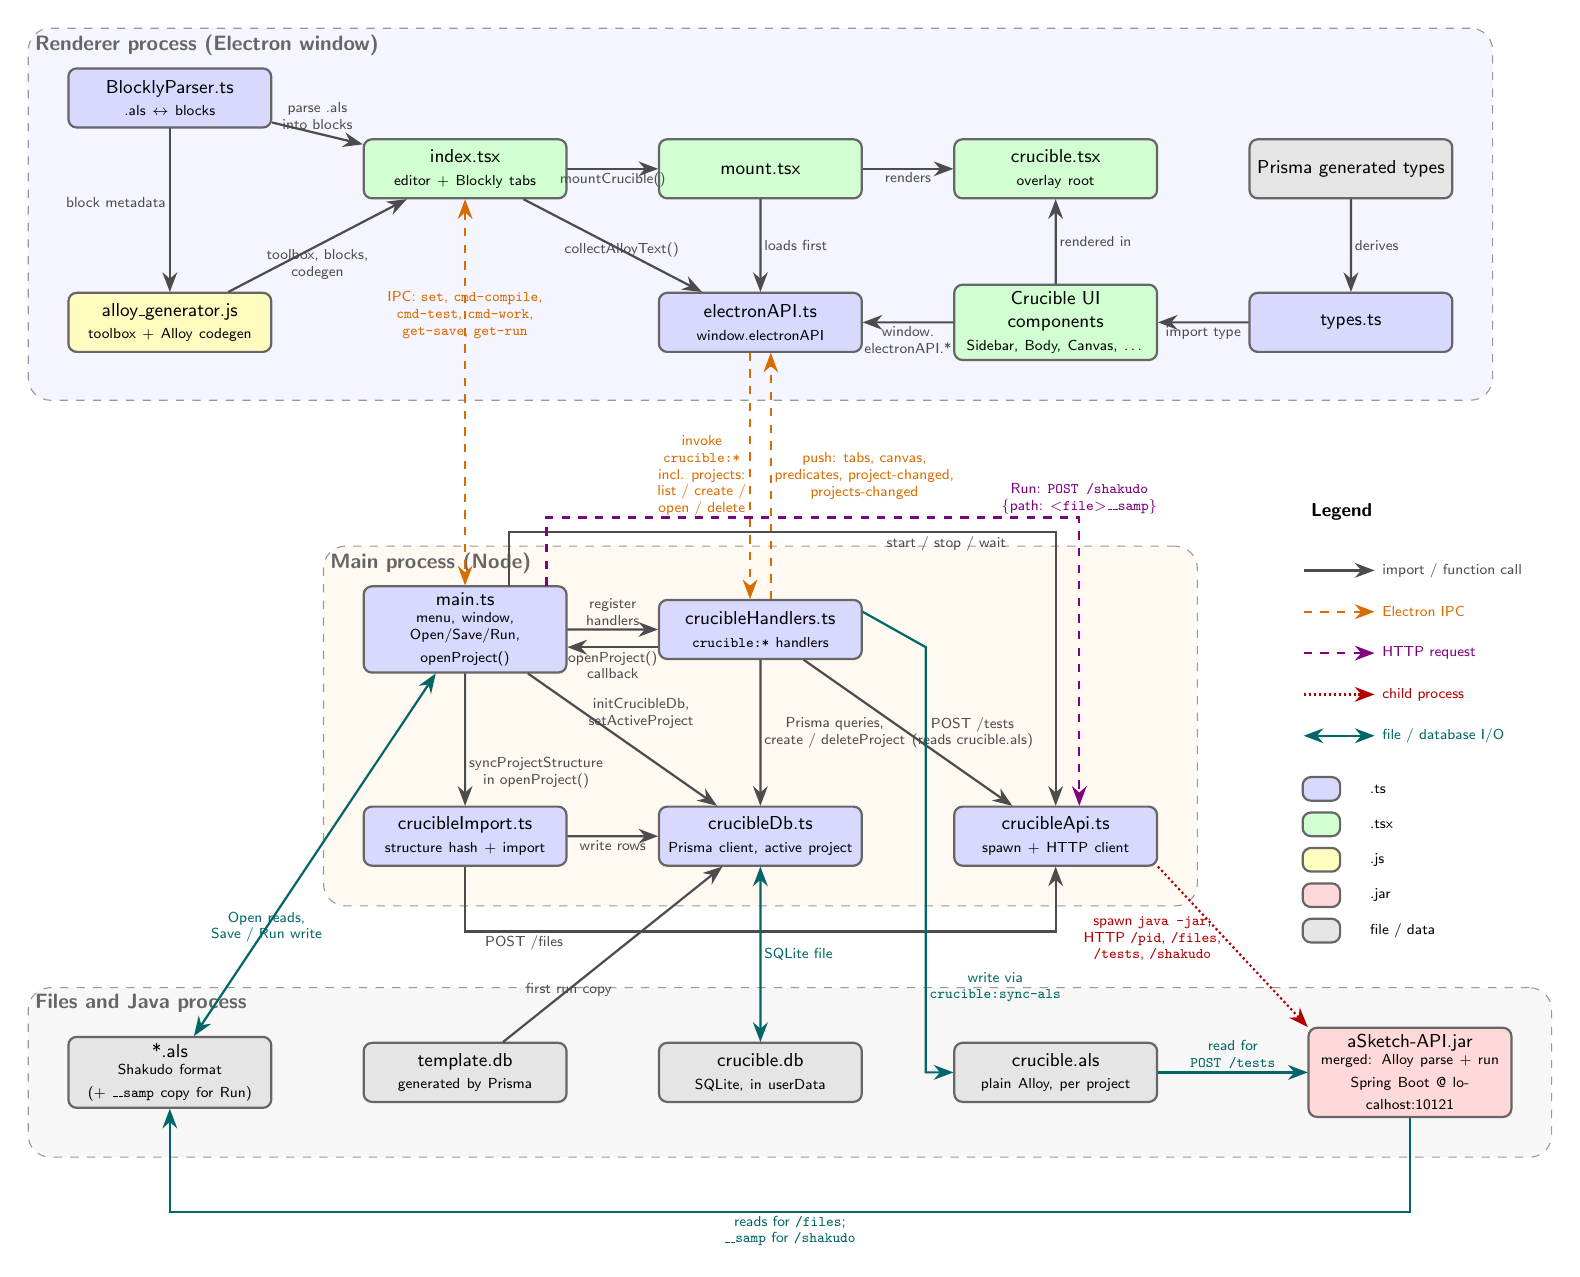
\begin{tikzpicture}[
  scale=0.75, every node/.append style={transform shape},
  >={Stealth[length=2.5mm]},
  box/.style={rectangle, rounded corners=3pt, draw=black!60, thick,
              minimum width=3.4cm, minimum height=1cm,
              text width=3.2cm, align=center, font=\sffamily\small},
  ts/.style={box, fill=blue!15},
  tsx/.style={box, fill=green!18},
  js/.style={box, fill=yellow!25},
  jar/.style={box, fill=red!15},
  file/.style={box, fill=gray!20},
  layer/.style={rectangle, rounded corners=8pt, draw=black!40, dashed,
                inner sep=0.5cm, fill=#1},
  layerlbl/.style={font=\sffamily\bfseries, text=black!60, anchor=north west},
  call/.style={->, thick, black!70},
  ipc/.style={->, thick, orange!85!black, dashed},
  http/.style={->, thick, violet, dashed},
  proc/.style={->, thick, red!70!black, densely dotted},
  data/.style={<->, thick, teal!80!black},
  lbl/.style={font=\sffamily\scriptsize, align=center, fill=none,
              fill opacity=0.9, text opacity=1, inner sep=1.5pt}
]

% ---------------- Renderer layer ----------------
\node[ts]  (parser) at (0,0)     {BlocklyParser.ts\\{\scriptsize .als $\leftrightarrow$ blocks}};
\node[js]  (gen)    at (0,-3.8)  {alloy\_generator.js\\{\scriptsize toolbox + Alloy codegen}};
\node[tsx] (index)  at (5,-1.2)  {index.tsx\\{\scriptsize editor + Blockly tabs}};
\node[tsx] (mount)  at (10,-1.2) {mount.tsx};
\node[tsx] (cruc)   at (15,-1.2) {crucible.tsx\\{\scriptsize overlay root}};
\node[ts]  (eapi)   at (10,-3.8) {electronAPI.ts\\{\scriptsize window.electronAPI}};
\node[tsx] (ui)     at (15,-3.8) {Crucible UI components\\{\scriptsize Sidebar, Body, Canvas, \dots}};
\node[ts]  (types)  at (20,-3.8) {types.ts};
\node[file](ptypes) at (20,-1.2) {Prisma generated types};

% ---------------- Main process layer ----------------
\node[ts]  (main)   at (5,-9)    {main.ts\\{\scriptsize menu, window, Open/Save/Run,\\openProject()}};
\node[ts]  (hand)   at (10,-9)   {crucibleHandlers.ts\\{\scriptsize \texttt{crucible:*} handlers}};
\node[ts]  (cimp)   at (5,-12.5) {crucibleImport.ts\\{\scriptsize structure hash + import}};
\node[ts]  (cdb)    at (10,-12.5){crucibleDb.ts\\{\scriptsize Prisma client, active project}};
\node[ts]  (capi)   at (15,-12.5){crucibleApi.ts\\{\scriptsize spawn + HTTP client}};

% ---------------- Files and Java layer ----------------
\node[file](als)    at (0,-16.5)  {*.als\\{\scriptsize Shakudo format\\(+ \texttt{\_\_samp} copy for Run)}};
\node[file](temp)   at (5,-16.5)  {template.db \\{\scriptsize generated by Prisma}};
\node[file](cdbf)   at (10,-16.5) {crucible.db\\{\scriptsize SQLite, in userData}};
\node[file](calsf)  at (15,-16.5) {crucible.als\\{\scriptsize plain Alloy, per project}};
\node[jar] (ajar)   at (21,-16.5) {aSketch-API.jar\\{\scriptsize merged: Alloy parse + run\\Spring Boot @ localhost:10121}};

% ---------------- Layer backgrounds ----------------
\begin{scope}[on background layer]
  \node[layer=blue!4, fit=(parser)(gen)(index)(mount)(cruc)(eapi)(ui)(types)(ptypes)] (L1) {};
  \node[layer=orange!5, fit=(main)(hand)(cimp)(cdb)(capi)] (L2) {};
  \node[layer=gray!6, fit=(als)(temp)(cdbf)(calsf)(ajar)] (L3) {};
\end{scope}
\node[layerlbl] at (L1.north west) {Renderer process (Electron window)};
\node[layerlbl] at (L2.north west) {Main process (Node)};
\node[layerlbl] at (L3.north west) {Files and Java process};

% ---------------- Renderer edges ----------------
\draw[call] (parser) -- node[lbl, above] {parse .als\\into blocks} (index);
\draw[call] (parser) -- node[lbl, pos=0.45, left] {block metadata} (gen);
\draw[call] (gen)    -- node[lbl, below] {toolbox, blocks,\\codegen} (index);
\draw[call] (index)  -- node[lbl, below] {mountCrucible()} (mount);
\draw[call] (mount)  -- node[lbl, below] {renders} (cruc);
\draw[call] (mount)  -- node[lbl, right] {loads first} (eapi);
\draw[call] (ui)     -- node[lbl, below] {window.\\electronAPI.*} (eapi);
\draw[call] (ui)     -- node[lbl, right] {rendered in} (cruc);
\draw[call] (types)  -- node[lbl, below] {import type} (ui);
\draw[call] (ptypes) -- node[lbl, right] {derives} (types);
\draw[call] (index)  -- node[lbl, pos=0.55] {collectAlloyText()} (eapi);

% ---------------- Cross-layer edges ----------------
% Shakudo IPC (both directions: menu actions down, invoke results up)
\draw[ipc, <->] (index.south) -- node[lbl, pos=0.3] {IPC: \texttt{set}, \texttt{cmd-compile},\\\texttt{cmd-test}, \texttt{cmd-work},\\\texttt{get-save}, \texttt{get-run}} (main.north);
% Crucible IPC, request and push
\draw[ipc] ([xshift=-5pt]eapi.south) -- node[lbl, left, pos=0.5]
  {invoke\\\texttt{crucible:*}\\incl. projects:\\list / create /\\open / delete} ([xshift=-5pt]hand.north);
\draw[ipc] ([xshift=5pt]hand.north) -- node[lbl, right, pos=0.5]
  {push: tabs, canvas,\\predicates, project-changed,\\projects-changed} ([xshift=5pt]eapi.south);

% ---------------- Main process edges ----------------
\draw[call] (main) -- node[lbl, pos=0.75, right] {syncProjectStructure\\in openProject()} (cimp);
\draw[call] (main) -- node[lbl, pos=0.3, right] {initCrucibleDb,\\setActiveProject} (cdb);
\draw[call] (main) -- node[lbl, above] {register \\handlers} (hand);
\draw[call] ([yshift=-0.3cm]hand.west) -- node[lbl, below] {openProject()\\callback} ([yshift=-0.3cm]main.east);
\draw[call] (hand) -- node[lbl, right] {Prisma queries,\\create / deleteProject} (cdb);
\draw[call] (cimp) -- node[lbl, below] {write rows} (cdb);
\draw[call] (cimp.south) -- ++(0,-1.1) -|
  node[lbl, pos=0.05, below] {POST /files} (capi.south);
\draw[call] (hand) -- node[lbl, right, pos=0.5] {POST /tests\\(reads crucible.als)} (capi);
\draw[call] (main.45) -- ++(0,0.9) -|
  node[lbl, pos=0.4, below] {start / stop / wait} (capi.north);
% Run: runs alongside start / stop / wait
\draw[http] ([xshift=-10pt]main.north east) -- ++(0,1.15) -|
  node[lbl, pos=0.5, above] {Run: \texttt{POST /shakudo}\\\{path: \texttt{\textless file\textgreater\_\_samp}\}} ([xshift=0.4cm]capi.north);

% ---------------- Files and Java edges ----------------
\draw[data] (als) -- node[lbl, pos=0.3] {Open reads,\\Save / Run write} (main);
\draw[data] (cdb) -- node[lbl, right] {SQLite file} (cdbf);
\draw[call] (temp) -- node[lbl, pos=0.3] {first run copy} (cdb);
\draw[proc] (capi.south east) -- node[lbl, left, pos=0.45] {spawn \texttt{java -jar};\\HTTP \texttt{/pid}, \texttt{/files},\\\texttt{/tests}, \texttt{/shakudo}} (ajar.north west);
\draw[->, thick, teal!80!black] ([yshift=0.3cm]hand.east) -- (12.8,-9.3) --
  node[lbl, pos=0.8, right] {write via\\\texttt{crucible:sync-als}} (12.8,-16.5) -- (calsf.west);
\draw[->, thick, teal!80!black] (calsf.east) -- node[lbl, above] {read for\\\texttt{POST /tests}} (ajar.west);
\draw[->, thick, teal!80!black] (ajar.south) -- ++(0,-1.6) -|
  node[lbl, pos=0.25, below] {reads for \texttt{/files};\\\texttt{\_\_samp} for \texttt{/shakudo}} (als.south);

% ---------------- Legend ----------------
\begin{scope}[shift={(19.2,-8)}]
  \node[font=\sffamily\small\bfseries, anchor=west] at (0,1) {Legend};
  \draw[call]  (0,0)    -- (1.2,0)    node[right, font=\sffamily\scriptsize] {import / function call};
  \draw[ipc]   (0,-0.7) -- (1.2,-0.7) node[right, font=\sffamily\scriptsize] {Electron IPC};
  \draw[http]  (0,-1.4) -- (1.2,-1.4) node[right, font=\sffamily\scriptsize] {HTTP request};
  \draw[proc]  (0,-2.1) -- (1.2,-2.1) node[right, font=\sffamily\scriptsize] {child process};
  \draw[data]  (0,-2.8) -- (1.2,-2.8) node[right, font=\sffamily\scriptsize] {file / database I/O};
  \node[ts,   minimum width=0.6cm, minimum height=0.4cm, text width=0.4cm] at (0.3,-3.7) {};
  \node[right, font=\sffamily\scriptsize] at (1.0,-3.7) {.ts};
  \node[tsx,  minimum width=0.6cm, minimum height=0.4cm, text width=0.4cm] at (0.3,-4.3) {};
  \node[right, font=\sffamily\scriptsize] at (1.0,-4.3) {.tsx};
  \node[js,   minimum width=0.6cm, minimum height=0.4cm, text width=0.4cm] at (0.3,-4.9) {};
  \node[right, font=\sffamily\scriptsize] at (1.0,-4.9) {.js};
  \node[jar,  minimum width=0.6cm, minimum height=0.4cm, text width=0.4cm] at (0.3,-5.5) {};
  \node[right, font=\sffamily\scriptsize] at (1.0,-5.5) {.jar};
  \node[file, minimum width=0.6cm, minimum height=0.4cm, text width=0.4cm] at (0.3,-6.1) {};
  \node[right, font=\sffamily\scriptsize] at (1.0,-6.1) {file / data};
\end{scope}

\end{tikzpicture}
\end{center}

\end{document}